Considerando la observación mencionada en la asignación de classroom, tomaremos la gráfica del ejercicio $7$ y usaremos la siguiente heurística
\begin{center}
    \begin{tabular}{c|cccccccc}
      & $s_0$ & $s_1$ & $s_2$ & $s_3$ & $s_4$ & $s_5$ & $s_6$ & $s_7$ \\
      \hline
      $h$ & $4$ & $15$ & $1$ & $0$ & $1$ & $0$ & $20$ & $0$ 
    \end{tabular}
  \end{center}

Donde el estado final será $s_7$ con $h(s_7)=0$, entonces se tiene la siguiente pila (cola de prioridad):
\begin{center}
    \begin{tabular}{|c|c|c|c|}
        \hline
        Estado actual & Siguientes estados & $f=g+h$ correspondiente & Cerrados\\
        \hline
        $s_0$ & $s_2$ & $4$ & $s_0$ \\
        \hline
        $s_2$ & $s_4, s_1$ & $3,21$ & $s_0,s_2$ \\
        \hline
        $s_4$ & $s_3, s_5, s_1$ & $6,10,21$ & $s_0,s_2,s_4$\\
        \hline
        $s_3$ & $s_5, s_1$ & $10,21$ & $s_0,s_2,s_4, s_3$\\
        \hline
        $s_5$ & $s_7, s_1, s_6$ & $20, 21, 32$ & $s_0,s_2,s_4, s_3, s_5$\\
        \hline
        $s_7$ & Estado final & NA & $s_0,s_2,s_4, s_3, s_5, s_7$\\
        \hline
    \end{tabular}
\end{center}
Con lo que tenemos el siguiente árbol:
\begin{center}
    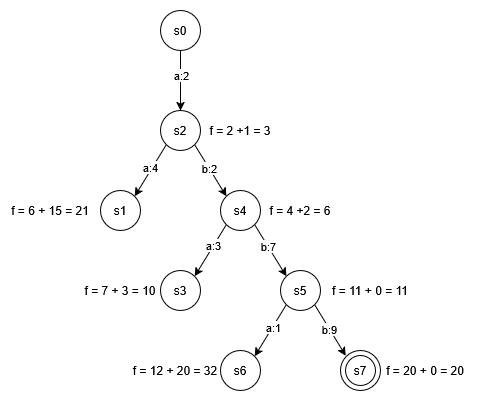
\includegraphics[height = 10cm]{respuestas/img/treeE6.png}
\end{center}

Por lo que el camino solución es $a,b,b,b$, donde se tiene los estados $s_0,s_2,s_4,s_5,s_7$. \\

Como observación, la heurística no es admisible ya que existe un camino de menor costo si de $s_5$ pasamos a $s_6$ y finalmente a $s_7$, sin embargo la  heurística de $s_6$ es muy alta.